\section{Weight Diagnostics}
\label{ssec:balancetables}

Table~\ref{tab:baltab1} displays the differences between the population-weighted mean covariate values of the non-expansion region and the weighted mean of the expansion region for our primary dataset and with the early expansion states excluded (calculated using our covariate adjustments). The weights presented here are from the H-SBW estimator. The values under each column of ``Primary'' and ``Early Excluded'' are in the following format: (unweighted difference, weighted difference). Additional results are available on request.

\begin{table}[ht]
\centering
    \caption{Balance Table}
    \label{tab:baltab1}
\begin{tabular}{lll}
  \hline
Variables & Preferred & Early expansion excluded \\ 
  \hline
age\_cat2\_19\_29\_pct & (0.35, 0.20) & (0.62, 0.07) \\ 
  age\_cat2\_30\_39\_pct & (-0.33, 0.16) & (0.11, 0.04) \\ 
  age\_cat2\_40\_49\_pct & (-0.22, 0.41) & (-0.04, 0.50) \\ 
  avg\_adult\_hh\_ratio & (-11.09, 0.40) & (-3.18, 0.18) \\ 
  citizenship\_pct & (3.56, 1.93) & (0.20, 1.80) \\ 
  disability\_pct & (1.46, -0.57) & (0.21, -0.73) \\ 
  educ\_hs\_degree\_pct & (3.35, -0.99) & (1.05, -1.14) \\ 
  educ\_less\_than\_hs\_pct & (0.40, -1.09) & (1.27, -1.27) \\ 
  educ\_some\_college\_pct & (0.30, -0.69) & (-0.44, -0.53) \\ 
  female\_pct & (0.34, 0.87) & (0.25, 1.00) \\ 
  foreign\_born\_pct & (-7.51, -1.99) & (-0.97, -1.99) \\ 
  hins\_unins\_pct\_2011 & (2.64, -0.48) & (3.09, -0.45) \\ 
  hins\_unins\_pct\_2012 & (3.37, 0.42) & (3.90, 0.42) \\ 
  hins\_unins\_pct\_2013 & (3.27, 0.32) & (3.77, 0.32) \\ 
  hispanic\_pct & (-4.36, -1.00) & (1.44, -1.00) \\ 
  inc\_pov2\_138\_pct & (2.08, -0.93) & (1.36, -0.60) \\ 
  inc\_pov2\_139\_299\_pct & (2.34, -0.91) & (1.45, -0.86) \\ 
  inc\_pov2\_300\_499\_pct & (0.80, 0.39) & (-0.05, 0.34) \\ 
  inc\_pov2\_500\_plus\_pct & (-5.69, 1.91) & (-3.06, 1.91) \\ 
  married\_pct & (0.80, 0.38) & (0.34, 0.60) \\ 
  missing\_children\_pct & (3.21, 0.36) & (1.93, 0.08) \\ 
  one\_child\_pct & (-0.80, 0.22) & (-0.21, 0.25) \\ 
  pop\_growth & (-0.11, 0.1) & (0.08, 0.15) \\ 
  race\_white\_pct & (3.87, -1.00) & (-0.31, -1.00) \\ 
  repub\_gov & (65.02, 22.06) & (55.02, 21.97) \\ 
  repub\_lower\_control & (74.91, 22.23) & (57.24, 20.66) \\ 
  repub\_total\_control & (73.72, 25.00) & (58.2, 25.00) \\ 
  student\_pct & (-0.29, 0.41) & (-0.12, 0.38) \\ 
  three\_plus\_child\_pct & (-0.02, 0.14) & (0.17, 0.15) \\ 
  two\_child\_pct & (-0.66, 0.47) & (-0.08, 0.55) \\ 
  unemployed\_pct\_2011 & (-0.80, -0.15) & (-0.68, -0.15) \\ 
  unemployed\_pct\_2012 & (-0.75, 0.00) & (-0.58, 0.00) \\ 
  unemployed\_pct\_2013 & (-0.29, 0.25) & (-0.10, 0.25) \\ 
  urban\_pct & (-0.08, 0.07) & (-0.03, 0.06) \\ 
   \hline
\end{tabular}
\end{table}

Table~\ref{tab:oatedist1} displays the difference in means from the overlap region from the control and treated regions on the primary dataset and with the early expansion states excluded. The numbers are displayed as (absolute distance from control region, absolute distance from treated region). These distances are computed using our adjusted datasets. 

\begin{table}[ht]
\centering
    \caption{Overlap region distance from control, treatment regions (1)}
    \label{tab:oatedist1}
\begin{tabular}{lll}
  \toprule
Variable & Preferred & Early expansion excluded \\ 
  \midrule
age\_cat2\_19\_29\_pct & (-1.39, -1.03) & (-1.34, -0.71) \\ 
  age\_cat2\_30\_39\_pct & (-0.79, -1.12) & (-0.82, -0.72) \\ 
  age\_cat2\_40\_49\_pct & (0.24, 0.02) & (0.2, 0.16) \\ 
  avg\_adult\_hh\_ratio & (-3.72, -14.81) & (-4.07, -7.25) \\ 
  citizenship\_pct & (1.7, 5.26) & (1.97, 2.17) \\ 
  disability\_pct & (0.29, 1.75) & (0.38, 0.59) \\ 
  educ\_hs\_degree\_pct & (1.14, 4.49) & (1.22, 2.27) \\ 
  educ\_less\_than\_hs\_pct & (-1.67, -1.27) & (-1.58, -0.31) \\ 
  educ\_some\_college\_pct & (0.47, 0.78) & (0.75, 0.31) \\ 
  female\_pct & (-0.11, 0.24) & (-0.16, 0.09) \\ 
  foreign\_born\_pct & (-2.23, -9.73) & (-2.8, -3.77) \\ 
  hins\_unins\_pct\_2011 & (-2.89, -0.24) & (-2.89, 0.19) \\ 
  hins\_unins\_pct\_2012 & (-3.68, -0.31) & (-3.68, 0.22) \\ 
  hins\_unins\_pct\_2013 & (-3.82, -0.55) & (-3.84, -0.07) \\ 
  hispanic\_pct & (-4.48, -8.84) & (-4.57, -3.13) \\ 
  inc\_pov2\_138\_pct & (-1.44, 0.64) & (-1.31, 0.05) \\ 
  inc\_pov2\_139\_299\_pct & (-0.18, 2.16) & (0, 1.45) \\ 
  inc\_pov2\_300\_499\_pct & (0.88, 1.68) & (0.96, 0.91) \\ 
  inc\_pov2\_500\_plus\_pct & (0.98, -4.71) & (0.58, -2.49) \\ 
  married\_pct & (1.6, 2.4) & (1.84, 2.18) \\ 
  missing\_children\_pct & (-0.72, 2.5) & (-0.62, 1.31) \\ 
  one\_child\_pct & (-0.27, -1.07) & (-0.32, -0.53) \\ 
  pop\_growth & (-0.27, -0.39) & (-0.29, -0.2) \\ 
  race\_white\_pct & (4.48, 8.35) & (5.15, 4.84) \\ 
  repub\_gov & (-11.88, 53.14) & (-11.94, 43.07) \\ 
  repub\_lower\_control & (-5.7, 69.21) & (-4.31, 52.92) \\ 
  repub\_total\_control & (-17.58, 56.14) & (-16.26, 41.94) \\ 
  student\_pct & (-0.5, -0.79) & (-0.5, -0.62) \\ 
  three\_plus\_child\_pct & (-0.17, -0.19) & (-0.1, 0.07) \\ 
  two\_child\_pct & (-0.15, -0.81) & (-0.16, -0.24) \\ 
  unemployed\_pct\_2011 & (0.09, -0.71) & (0.08, -0.6) \\ 
  unemployed\_pct\_2012 & (0.05, -0.69) & (0.02, -0.55) \\ 
  unemployed\_pct\_2013 & (-0.42, -0.71) & (-0.44, -0.54) \\ 
  urban\_pct & (-0.05, -0.13) & (-0.05, -0.08) \\ 
   \bottomrule
\end{tabular}
\end{table}

Figure~\ref{fig:sbwvhsbw} shows the sum of the SBW weights by state versus the H-SBW weights on our primary dataset with our preferred estimator. We see that the H-SBW more evenly disperses the weights across states relative to SBW. This can be desirable if we believe there are positive dependencies within state in the outcome model.

\begin{figure}[]
\begin{center}
    \caption{H-SBW versus SBW weights}
    \label{fig:corrmatrix}
    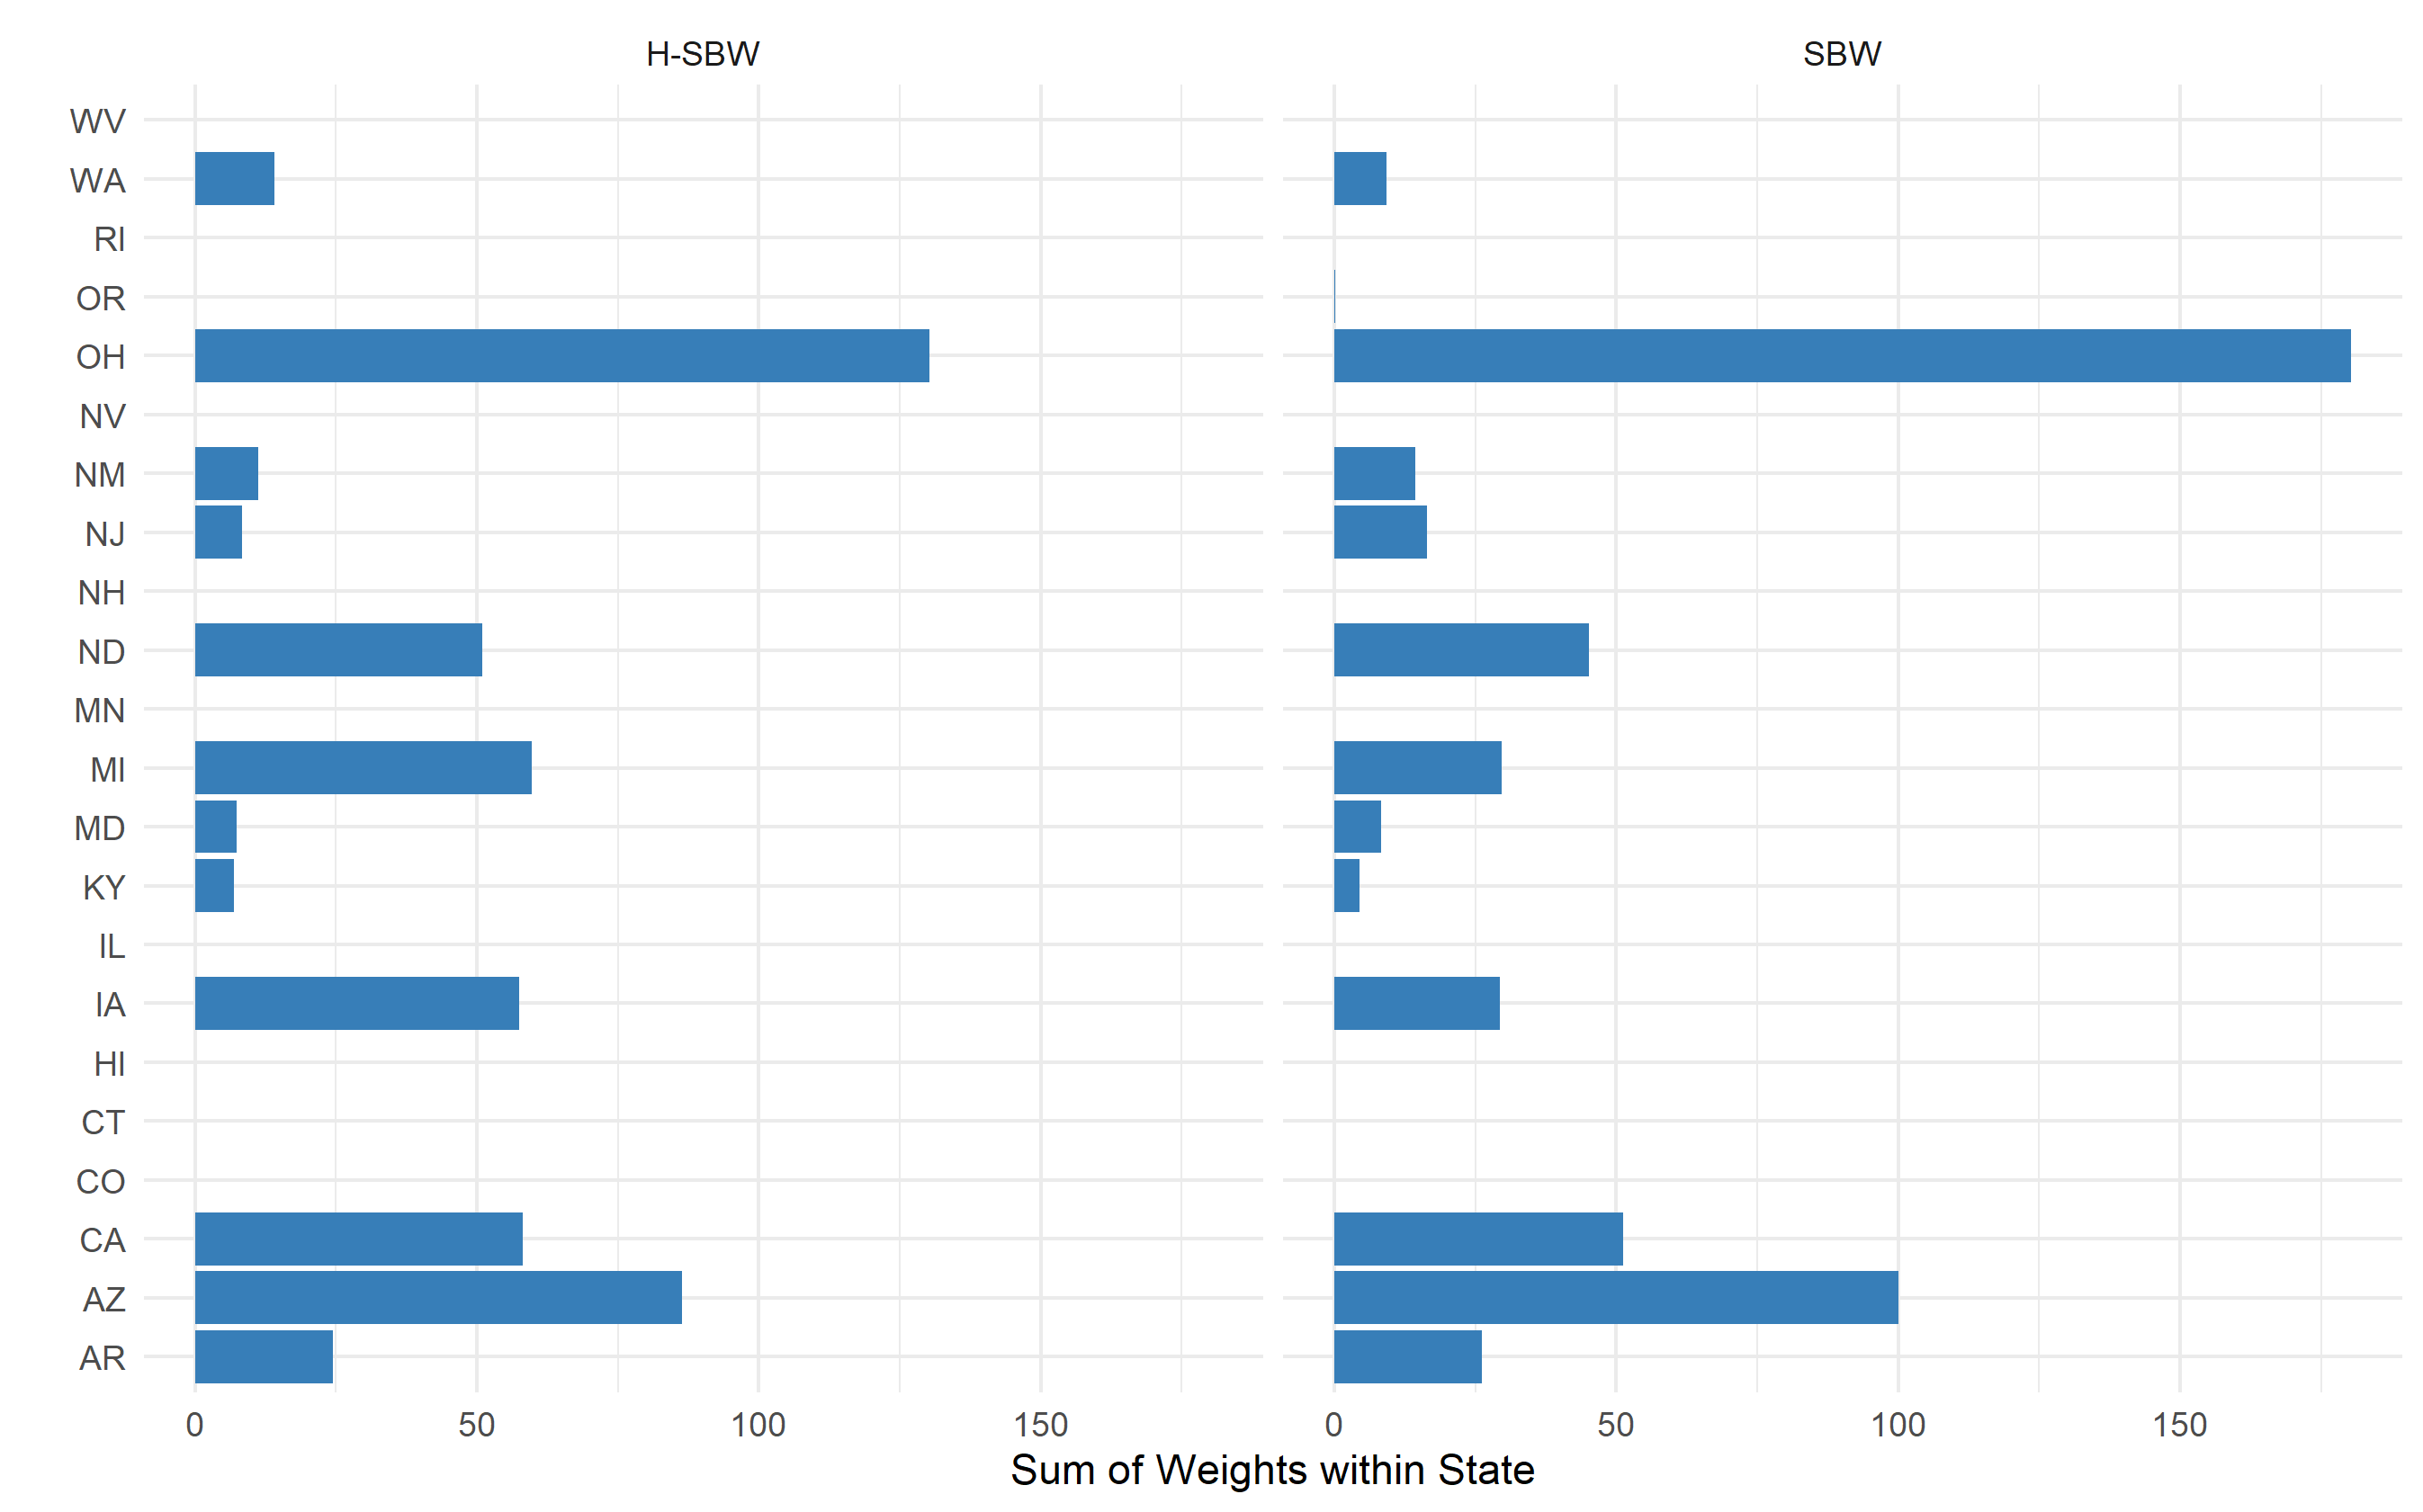
\includegraphics[scale=0.6]{01_Plots/weights-by-state-sbw-hsbw-c1.png}
\end{center}
\end{figure}

Table ~\ref{tab:oatestateweightsc1} displays the sum of CPUMA-level weights within each state for the OATE region, using the preferred covariate adjustment (``sigma\_uu\_i''), as well as no adjustment (``sigma\_zero'') and the secondary adjustment (``sigma\_uu\_avg''). We display all states where the total sum of weights within states is greater than one for any state. The total sum of weights for each set is standardized to sum to 100 for each set of weights. Table ~\ref{tab:oatestateweightsc2} displays the same results with the early expansion states excluded.

\begin{table}[ht]
\centering
\caption{OATE weights summed by state by covariate adjustment, primary dataset}
\label{tab:oatestateweightsc1}
\begin{tabular}{lrrrr}
  \hline
State & Treatment & sigma\_uu\_i & sigma\_uu\_avg & sigma\_zero \\ 
  \hline
CA & 1 & 25.95 & 25.69 & 21.29 \\ 
  OH & 1 & 22.27 & 21.26 & 22.08 \\ 
  AL & 0 & 13.78 & 13.54 & 10.39 \\ 
  OR & 1 & 12.36 & 12.87 & 12.62 \\ 
  FL & 0 & 11.21 & 11.96 & 11.66 \\ 
  WI & 0 & 10.99 & 11.16 & 10.23 \\ 
  MO & 0 & 10.44 & 10.34 & 10.90 \\ 
  PA & 0 & 9.28 & 10.40 & 10.33 \\ 
  LA & 0 & 9.10 & 9.23 & 11.12 \\ 
  IL & 1 & 8.51 & 9.40 & 8.58 \\ 
  KS & 0 & 7.11 & 7.05 & 5.89 \\ 
  MN & 1 & 6.56 & 5.81 & 7.22 \\ 
  TX & 0 & 6.18 & 4.70 & 4.72 \\ 
  MD & 1 & 5.80 & 6.04 & 7.65 \\ 
  KY & 1 & 4.64 & 4.75 & 4.59 \\ 
  NE & 0 & 3.84 & 4.24 & 4.32 \\ 
  IN & 0 & 3.80 & 3.33 & 3.39 \\ 
  AZ & 1 & 3.52 & 3.05 & 4.11 \\ 
  AR & 1 & 3.31 & 3.61 & 3.82 \\ 
  ME & 0 & 3.24 & 3.12 & 3.23 \\ 
  RI & 1 & 2.66 & 3.06 & 3.09 \\ 
  NC & 0 & 2.34 & 2.20 & 3.36 \\ 
  SC & 0 & 2.23 & 2.83 & 1.95 \\ 
  NH & 1 & 2.16 & 1.35 & 1.22 \\ 
  OK & 0 & 2.08 & 1.70 & 2.60 \\ 
  GA & 0 & 1.67 & 1.70 & 1.91 \\ 
  WA & 1 & 1.46 & 1.95 & 1.95 \\ 
  MS & 0 & 0.88 & 1.12 & 0.54 \\ 
  VA & 0 & 0.84 & 0.59 & 1.74 \\ 
  TN & 0 & 0.59 & 0.50 & 1.01 \\ 
  NJ & 1 & 0.37 & 0.36 & 0.48 \\ 
  WY & 0 & 0.37 & 0.20 & 0.45 \\ 
  ND & 1 & 0.35 & 0.64 & 1.06 \\ 
   \hline
\end{tabular}
\end{table}

\begin{table}[ht]
\centering
\caption{OATE weights summed by state by covariate adjustment, early expansion excluded}
\label{tab:oatestateweightsc2}
\begin{tabular}{lrrrr}
  \hline
State & Treatment & sigma\_uu\_i & sigma\_uu\_avg & sigma\_zero \\ 
  \hline
FL & 0 & 29.59 & 29.53 & 26.90 \\ 
  CO & 1 & 29.36 & 29.58 & 24.95 \\ 
  IL & 1 & 13.23 & 14.66 & 13.82 \\ 
  HI & 1 & 11.57 & 11.54 & 9.98 \\ 
  MD & 1 & 9.67 & 10.23 & 13.33 \\ 
  WI & 0 & 9.11 & 9.21 & 8.33 \\ 
  PA & 0 & 8.69 & 9.52 & 10.42 \\ 
  MO & 0 & 8.36 & 8.86 & 9.12 \\ 
  OH & 1 & 8.32 & 6.63 & 8.33 \\ 
  AZ & 1 & 6.99 & 6.53 & 7.37 \\ 
  NC & 0 & 6.91 & 7.16 & 7.37 \\ 
  KY & 1 & 6.86 & 6.78 & 6.43 \\ 
  AR & 1 & 5.95 & 6.18 & 6.04 \\ 
  IN & 0 & 5.21 & 5.18 & 5.50 \\ 
  ME & 0 & 3.81 & 3.53 & 2.85 \\ 
  AL & 0 & 3.79 & 3.44 & 3.72 \\ 
  LA & 0 & 3.71 & 3.21 & 3.98 \\ 
  MS & 0 & 3.38 & 3.28 & 4.06 \\ 
  TN & 0 & 2.97 & 3.70 & 3.47 \\ 
  TX & 0 & 2.61 & 2.08 & 2.66 \\ 
  ND & 1 & 2.56 & 2.47 & 1.62 \\ 
  GA & 0 & 2.29 & 2.61 & 2.41 \\ 
  VA & 0 & 2.06 & 1.31 & 2.22 \\ 
  NV & 1 & 1.81 & 1.17 & 2.67 \\ 
  SC & 0 & 1.63 & 1.29 & 1.03 \\ 
  NH & 1 & 1.48 & 1.75 & 2.02 \\ 
  NM & 1 & 1.41 & 1.37 & 2.16 \\ 
  MT & 0 & 1.40 & 1.31 & 0.91 \\ 
  KS & 0 & 1.33 & 1.67 & 1.30 \\ 
  OK & 0 & 1.07 & 1.03 & 1.51 \\ 
  UT & 0 & 0.88 & 0.90 & 1.06 \\ 
   \hline
\end{tabular}
\end{table}
